
El volumen de datos textuales digitalizados generados diariamente, provenientes de fuentes como la web, redes sociales, registros médicos y libros digitalizados, es simplemente enorme. Como resultado, se ha vuelto imperativo traducir, analizar y gestionar esta avalancha de palabras y texto.

El Procesamiento del Lenguaje Natural (PLN) es el campo que se encarga de diseñar métodos y algoritmos que trabajan con datos de lenguaje natural, ya sea como entrada o salida \cite{goldberg2017neural}. El objetivo principal del PLN es desarrollar y analizar algoritmos computacionales y representaciones para procesar el lenguaje humano de manera efectiva \cite{jacobbook}.

Es importante destacar que el lenguaje natural puede provenir tanto de fuentes escritas como habladas. Aunque el PLN suele centrarse más en el procesamiento de texto, se pueden aplicar técnicas de reconocimiento de habla o transcripción para abordar de manera similar ambas fuentes de información.

\section{Desafíos del Procesamiento del Lenguaje Natural (PLN)}

A continuación, se discuten varias propiedades del lenguaje humano que hacen extremadamente complejo cumplir con los objetivos del PLN.

\paragraph{Ambigüedad}

El lenguaje humano es sumamente ambiguo. Tomemos, por ejemplo, las siguientes oraciones:

\begin{enumerate}
  \item ``Yo comí pizza con amigos.''
  \item ``Yo comí pizza con aceitunas.''
  \item ``Yo comí pizza con un tenedor.''
\end{enumerate}

Aunque las tres oraciones tienen una estructura gramatical muy similar, difieren en cómo las frases nominales siguientes a la preposición ``con'' se relacionan con las partes anteriores. En la primera oración, ``amigos'' modifica al pronombre ``yo''; en la segunda, ``aceitunas'' modifica a la pizza; y en la tercera, ``un tenedor'' modifica al verbo ``comer''. Para realizar estas distinciones, es necesario tener en cuenta el contexto situacional, lo cual puede resultar natural para una persona, pero muy complejo para una máquina.

\paragraph{Dinamismo}

El lenguaje está en constante cambio y evolución. Siempre surgen nuevas palabras o se les asignan nuevos significados, mientras que otras palabras caen en desuso. Las redes sociales, por ejemplo, pueden acelerar este proceso, como ocurre con los hashtags en Twitter.

\paragraph{Discretitud}

El lenguaje escrito, como una oración o un documento, se puede entender como una secuencia de palabras discretas provenientes de un vocabulario finito. La naturaleza discreta de las palabras implica que no podemos inferir la relación entre dos palabras basándonos únicamente en las letras que las componen. Por ejemplo, las palabras ``hamburguesa'', ``pizza'' y ``tiza'', aunque las dos primeras están más cerca entre sí semánticamente, las dos últimas tienen una mayor similitud en cuanto a las letras que las forman.

\paragraph{Composicionalidad}
El significado de una oración va más allá del significado individual de sus palabras. Esto implica que, aunque tengamos formas de representar computacionalmente el significado de las palabras, esto no garantiza que podamos representar cómo se componen para formar significados a nivel de oración.

\paragraph{Dispersión (sparseness)}

La forma en que las palabras (símbolos discretos) pueden combinarse para formar significados es prácticamente infinita. Esto implica que, en general, las oraciones que encontramos en un documento son únicas o rara vez han sido escritas antes. Por lo tanto, cualquier enfoque de fuerza bruta que intente memorizar oraciones a partir de una coleccion de documentos data (o corpus) no garantiza una buena generalización a textos nuevos.






\section{PLN y Lingüística Computacional}

El Procesamiento del Lenguaje Natural (PLN) a menudo se confunde con otra disciplina relacionada llamada Lingüística Computacional (LC). Aunque están estrechamente vinculadas, tienen enfoques distintos. La LC busca abordar preguntas fundamentales sobre el lenguaje utilizando la computación, investigando cómo entendemos, producimos y aprendemos lenguaje. En este sentido, la LC se acerca más a la lingüística, cuyo objeto de estudio es el lenguaje humano, apoyándose en métodos computacionales, de manera similar a la biología computacional o la astronomía computacional.

Por otro lado, en el PLN el enfoque está en resolver tareas específicas, como la transcripción automática del habla, la traducción automática, la extracción de información de documentos y el análisis de opiniones en redes sociales. Es importante señalar que en el PLN, el éxito de una solución se mide en función de métricas concretas, como la similitud de una traducción automática con una realizada por un humano, independientemente de si el modelo utiliza alguna teoría lingüística. Si bien los conocimientos lingüísticos fundamentales pueden ser cruciales para llevar a cabo estas tareas, el éxito se evalúa en función de si se logra o no el objetivo establecido, de acuerdo con una métrica de evaluación \cite{jacobbook}.

\section{Tareas en Procesamiento del Lenguaje Natural (PLN)}

El procesamiento del lenguaje natural (PLN) desarrolla métodos para resolver problemas prácticos relacionados con el lenguaje \cite{JohnsonMLSS}. A estos problemas se les suele llamar ``tareas'' o ``tasks'' en inglés. Cada tarea define formalmente la entrada (input) y salida (output) esperada de un sistema de PLN.

A continuación, se presentan algunos ejemplos de estas tareas junto con sus nombres en inglés:

\begin{itemize}
  \item \textbf{Reconocimiento automático del habla (Speech Recognition)}: La entrada es una señal de audio con voz y la salida es texto escrito.
  \item \textbf{Traducción automática (Machine Translation)}: La entrada es texto en el idioma fuente y la salida es texto en el idioma destino.
  \item \textbf{Extracción de información de documentos (Information Extraction)}: La entrada es texto libre y la salida es una tabla estructurada que contiene la información extraída del texto.
  \item \textbf{Clasificación de texto (Text Classification)}: La entrada es texto libre y la salida es la asignación a una categoría discreta dentro de un conjunto finito de categorías.
  \item \textbf{Extracción de Entidades Nombradas (Named Entity Recognition, NER)}: La entrada es una oración y la salida es la marcación de las entidades identificadas en la oración, como personas, lugares u organizaciones, como se muestra en la Figura \ref{fig:ner}.
  \item \textbf{Respuestas a Preguntas (Question Answering)}: La entrada es una pregunta y la salida es una respuesta.
  \item \textbf{Comprensión de Lectura (Reading Comprehension)}: La entrada es un pasaje de texto y una pregunta, y la salida es la ubicación marcada donde se encuentra la respuesta correcta dentro del pasaje proporcionado.
  \item \textbf{Etiquetado Gramatical (Part-of-Speech Tagging)}: La entrada es una oración y la salida son las categorías gramaticales (por ejemplo, verbo, sustantivo, adjetivo) de las palabras dentro de la oración.
  \item \textbf{Extracción de Resúmenes (Summarization)}: La entrada es un documento y la salida es un párrafo que resume su contenido.
\end{itemize}

\begin{figure}[h]
	\centering
	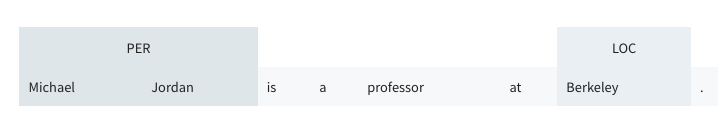
\includegraphics[scale=0.4]{pics/NER.png}
	\caption{Reconocimiento de Entidades Nombradas}
	\label{fig:ner}
\end{figure}
\section{Niveles de descripción lingüística}

El campo de la \textbf{descripción lingüística} abarca diferentes niveles:

\begin{itemize}
  \item \textbf{Fonética y fonología:} estudio de los sonidos del habla.
  \item \textbf{Morfología:} estudio de la estructura de las palabras.
  \item \textbf{Sintaxis:} estudio de la estructura de las oraciones.
  \item \textbf{Semántica:} estudio del significado de las palabras y oraciones.
  \item \textbf{Pragmática:} estudio del uso del lenguaje en el contexto.
\end{itemize}

El PLN puede abordar tareas en cada uno de estos niveles, pero a menudo se enfoca en niveles más altos de representación y comprensión.




\subsection{Fonética}

La fonética es la rama de la lingüística que se ocupa del estudio de los sonidos del lenguaje. Examina los órganos utilizados en la producción de sonidos, como la boca, la lengua, la garganta, la nariz, los labios y el paladar. Los sonidos del lenguaje se dividen en vocales y consonantes. Las vocales se producen con poca restricción del flujo de aire desde los pulmones, mientras que las consonantes implican alguna restricción o cierre en el tracto vocal \cite{JohnsonMLSS, fromkin2018introduction}. Además, el Alfabeto Fonético Internacional (AFI) proporciona una notación alfabética para representar los sonidos fonéticos.

\subsection{Fonología}

La fonología se centra en el estudio de cómo los sonidos del habla forman patrones y construyen significado. Los fonemas son las unidades básicas de sonido que diferencian el significado de las palabras. Por ejemplo, en inglés, la "p" y la "b" son fonemas distintos porque cambian el significado de las palabras en las que se encuentran. La fonología también examina las variaciones en la pronunciación de los sonidos en diferentes contextos y dialectos \cite{fromkin2018introduction}.

\subsection{Morfología}

La morfología se ocupa del estudio de la estructura interna de las palabras. Los morfemas son las unidades mínimas de significado que componen las palabras. Por ejemplo, en la palabra "deshacer", los morfemas son "des-", "hacer" y "-er". La morfología también se interesa por los procesos de formación de palabras, como la derivación, donde se agregan prefijos o sufijos a una palabra existente para formar una nueva palabra con un significado diferente \cite{JohnsonMLSS}.

\begin{itemize}
\item La morfología estudia la estructura de las palabras (por ejemplo, re+estructur+ando, in+olvid+able) \cite{JohnsonMLSS}
\item Morfema: el término lingüístico para la unidad más elemental de forma gramatical \cite{fromkin2018introduction}. Por ejemplo, morfología = morf + ología (la ciencia de).
\item Morfología derivativa: proceso de formar una nueva palabra a partir de una palabra existente, a menudo mediante la adición de un prefijo o sufijo.
\item La morfología derivativa exhibe una estructura jerárquica. Ejemplo: re+vital+iz+ación
\begin{figure}[h]
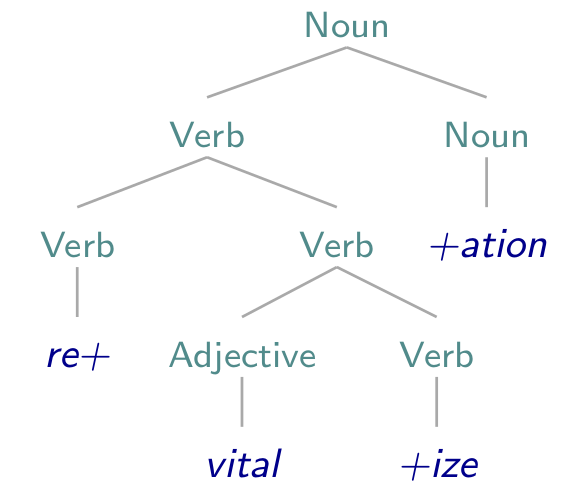
\includegraphics[scale = 0.2]{pics/morphology.png}
\end{figure}
\item El sufijo generalmente determina la categoría sintáctica (part-of-speech) de la palabra derivada.
\end{itemize}

\subsection{Sintaxis}

La sintaxis es el estudio de cómo las palabras se combinan para formar frases y oraciones gramaticales. Examina las reglas y estructuras que determinan la organización de las palabras en una oración y cómo influyen en el significado. La sintaxis también se ocupa de la relación entre las palabras y las funciones que desempeñan dentro de una oración. Por ejemplo, en la oración "El perro persigue al gato", "el perro" es el sujeto, "persigue" es el verbo y "al gato" es el complemento directo \cite{JohnsonMLSS}.

\begin{itemize}
\item La sintaxis estudia las formas en que las palabras se combinan para formar frases y oraciones \cite{JohnsonMLSS}
\begin{figure}[h]
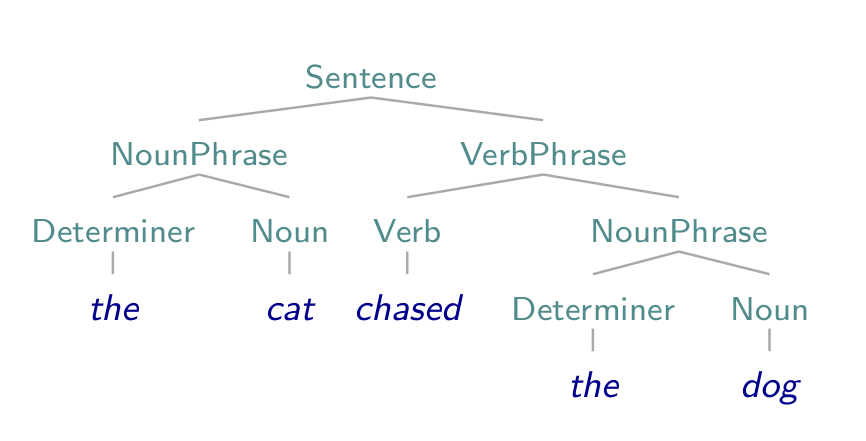
\includegraphics[scale = 0.3]{pics/parseTree1.png}
\end{figure}
\item El análisis sintáctico ayuda a identificar \textbf{quién hizo qué a quién}, un paso clave para comprender una oración.
\end{itemize}


\subsection{Semántica}

La semántica es el estudio del significado de las palabras, frases y oraciones, examinando cómo se construye e interpreta este significado en el contexto del lenguaje. Además, la semántica se interesa por los roles semánticos, que indican la función de cada entidad en una oración. Por ejemplo, en la oración "El niño cortó la cuerda con una navaja", "el niño" es el agente, "la cuerda" es el tema y "una navaja" es el instrumento \cite{JohnsonMLSS}.

La semántica se enfoca en el significado de las palabras, frases y oraciones. Estudia cómo se construye e interpreta este significado en el contexto del lenguaje. Además, dentro de la semántica, se analizan los roles semánticos, los cuales indican la función que desempeña cada entidad en una oración. Por ejemplo, en la oración "El niño cortó la cuerda con una navaja", se identifican distintos roles semánticos: "el niño" como el agente, "la cuerda" como el tema y "una navaja" como el instrumento utilizado \cite{JohnsonMLSS}.


En resumen:
\begin{itemize}
\item La semántica estudia el significado de las palabras, frases y oraciones \cite{JohnsonMLSS}.
\item Dentro de la semántica, se analizan los roles semánticos, que indican el papel desempeñado por cada entidad en una oración.
\item Algunos ejemplos de roles semánticos son: \textcolor[rgb]{0.00,0.00,1.00}{\textbf{agente}} (la entidad que realiza la acción), \textcolor[rgb]{1.00,0.00,0.00}{\textbf{tema}} (la entidad involucrada en la acción) y \textcolor[rgb]{0.00,1.00,0.00}{\textbf{instrumento}} (otra entidad utilizada por el agente para llevar a cabo la acción).
\item En la oración "El niño cortó la cuerda con una navaja", se puede identificar el agente como \textcolor[rgb]{0.00,0.00,1.00}{\textbf{el niño}}, el tema como \textcolor[rgb]{1.00,0.00,0.00}{\textbf{la cuerda}} y el instrumento como \textcolor[rgb]{0.00,1.00,0.00}{\textbf{una navaja}}.
\item Además de los roles semánticos, la semántica también abarca las relaciones léxicas, que son las relaciones entre diferentes palabras \cite{yule2016study}.
\item Algunos ejemplos de relaciones léxicas incluyen la sinonimia (conceal/hide), la antonimia (shallow/deep) y la hiponimia (perro/animal).
\end{itemize}


\subsection{Pragmática}

La pragmática se centra en cómo el contexto influye en la interpretación y el significado de las expresiones lingüísticas. Examina cómo se utilizan las expresiones lingüísticas en situaciones reales y cómo los hablantes interpretan el significado implícito. Por ejemplo, la oración "Hace frío aquí" puede interpretarse como una sugerencia implícita de cerrar las ventanas \cite{fromkin2018introduction}.


\section{Procesamiento del Lenguaje Natural y Aprendizaje Automático}

Comprender y producir el lenguaje computacionalmente es extremadamente complejo.  La tecnología más exitosa actualmente para abordar PLN es el aprendizaje automático supervisado que consiste en una familia de algoritmos que “aprenden” a construir la respuesta del problema en cuestión en base a encontrar patrones en datos de entrenamiento etiquetados. Por ejemplo, si queremos tener un modelo que nos diga si un tweet tiene un sentimiento positivo o negativo respecto a un producto, primero necesito  etiquetar manualmente un conjunto de tweets con su sentimiento asociado. Luego debo entrenar un algoritmo de aprendizaje sobre estos datos para poder predecir de manera automática el sentimiento asociado a tweets desconocidos. Como se podrán imaginar, el etiquetado de datos es una parte fundamental de la solución y puede ser un proceso muy costoso, especialmente cuando se requiere conocimiento especializado para definir la etiqueta.

La esencia del aprendizaje automático supervisado es la creación de mecanismos que puedan examinar ejemplos y producir generalizaciones \cite{goldberg2017neural}. Diseñamos un algoritmo cuya entrada es un conjunto de ejemplos etiquetados y cuya salida es una función (o un programa) que recibe una instancia y produce la etiqueta deseada. Por ejemplo, si la tarea es distinguir entre correos electrónicos de spam y no spam, los ejemplos etiquetados serían correos electrónicos etiquetados como spam y correos electrónicos etiquetados como no spam. Se espera que la función resultante produzca predicciones de etiquetas correctas también para instancias que no ha visto durante el entrenamiento. Este enfoque difiere de diseñar un algoritmo para realizar la tarea (por ejemplo, sistemas basados en reglas diseñados manualmente).



Aunque los seres humanos somos grandes usuarios del lenguaje, también somos muy malos para comprender y describir formalmente las reglas que rigen el lenguaje.

Entender y producir lenguaje utilizando computadoras es altamente desafiante. Los métodos más conocidos para lidiar con datos de lenguaje se basan en el aprendizaje automático supervisado.

El aprendizaje automático supervisado consiste en intentar inferir patrones y regularidades a partir de un conjunto de pares de entrada y salida preanotados (también conocido como conjunto de datos de entrenamiento).

\paragraph{Conjunto de Datos de Entrenamiento: Datos de NER CoNLL-2003}

Cada línea contiene un token, una etiqueta de parte de la oración, una etiqueta de sintagma y una etiqueta de entidad nombrada.
\begin{center}
\begin{verbatim}
U.N.         NNP  I-NP  I-ORG
official     NN   I-NP  O
Ekeus        NNP  I-NP  I-PER
heads        VBZ  I-VP  O
for          IN   I-PP  O
Baghdad      NNP  I-NP  I-LOC
.            .    O     O
\end{verbatim}
\end{center}

\footnotemark{Fuente: \url{https://www.clips.uantwerpen.be/conll2003/ner/}}


\subsection{Ejemplo 1: Clasificación de temas}

La clasificación de temas es una tarea de Procesamiento del Lenguaje Natural (PLN) en la cual se asigna a un documento una de varias categorías, como deportes, política, cotilleos o economía. Las palabras presentes en los documentos brindan pistas importantes sobre su tema. Sin embargo, redactar reglas para esta tarea es un desafío debido a la complejidad del lenguaje. La anotación de datos, en la cual los lectores clasifican los documentos por temas, puede ayudar a generar conjuntos de datos de entrenamiento para algoritmos de aprendizaje automático supervisado. Estos algoritmos aprenden patrones de uso de palabras que facilitan la categorización de los documentos.

\begin{itemize}
\item Clasificar un documento en una de las cuatro categorías: Deportes, Política, Cotilleos y Economía.
\item Las palabras en los documentos proporcionan indicios muy sólidos.
\item ¿Qué palabras brindan qué indicios?
\item Elaborar reglas para esta tarea resulta bastante desafiante.
\item No obstante, los lectores pueden categorizar fácilmente varios documentos según su tema (anotación de datos).
\item Un algoritmo de aprendizaje automático supervisado puede identificar los patrones de uso de palabras que ayudan a categorizar los documentos.
\end{itemize}


\subsection{Ejemplo 2: Análisis de Sentimiento}

El análisis de sentimientos se refiere a la aplicación de técnicas de Procesamiento del Lenguaje Natural (PLN) para identificar y extraer información subjetiva de conjuntos de datos textuales. Un desafío común en el análisis de sentimientos es la clasificación de la polaridad a nivel de mensaje (MPC), donde las frases se clasifican automáticamente en categorías positivas, negativas o neutrales. Las soluciones más avanzadas utilizan modelos de aprendizaje automático supervisado entrenados con ejemplos anotados manualmente.

En este tipo de clasificación, es habitual emplear el aprendizaje supervisado, siendo las Máquinas de Vectores de Soporte (SVM) una opción popular. El objetivo de las SVM es encontrar un hiperplano que separe las clases con el margen máximo, logrando la mejor separación entre las clases positivas, negativas y neutrales \cite{jacobbook}.

\begin{itemize}
  \item Aplicación de técnicas de \textbf{PLN} para identificar y extraer información subjetiva de conjuntos de datos textuales.
  \item Clasificación automática de frases en las categorías \textcolor[rgb]{0.00,0.00,1.00}{\textbf{positiva}}, \textcolor[rgb]{1.00,0.00,0.00}{\textbf{negativa}} o \textcolor[rgb]{0.00,1.00,0.00}{\textbf{neutral}}.

     \begin{figure}[h]
        	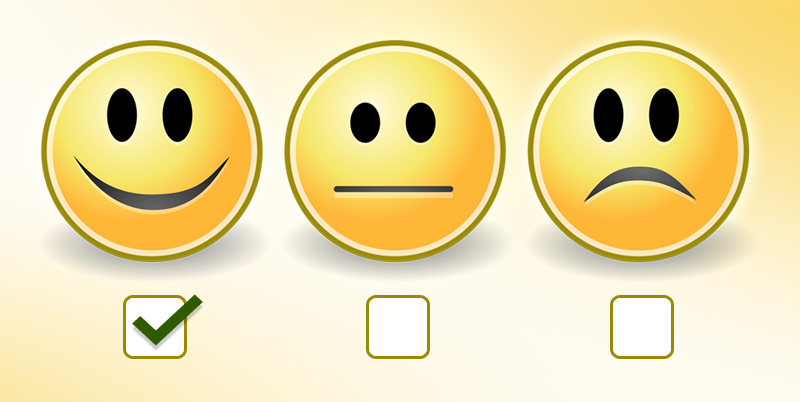
\includegraphics[scale = 0.15]{pics/sent.png}
        \end{figure}

  \item Las soluciones más avanzadas emplean modelos de aprendizaje automático \textbf{supervisado}, entrenados con ejemplos \textbf{anotados manualmente} \cite{Mohammad2013}.
\end{itemize}


\begin{figure}[h]
        	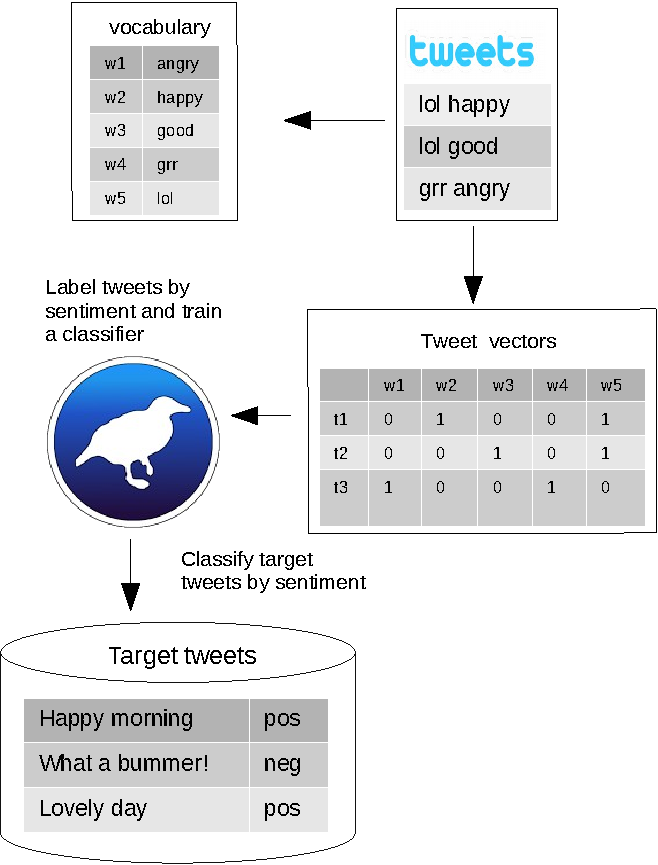
\includegraphics[scale = 0.5]{pics/bagOfwordsClassification.pdf}
        \end{figure}


\begin{itemize}


\item Idea: Encontrar un hiperplano que separe las clases con el margen máximo (mayor separación).

     \begin{figure}[h]
        	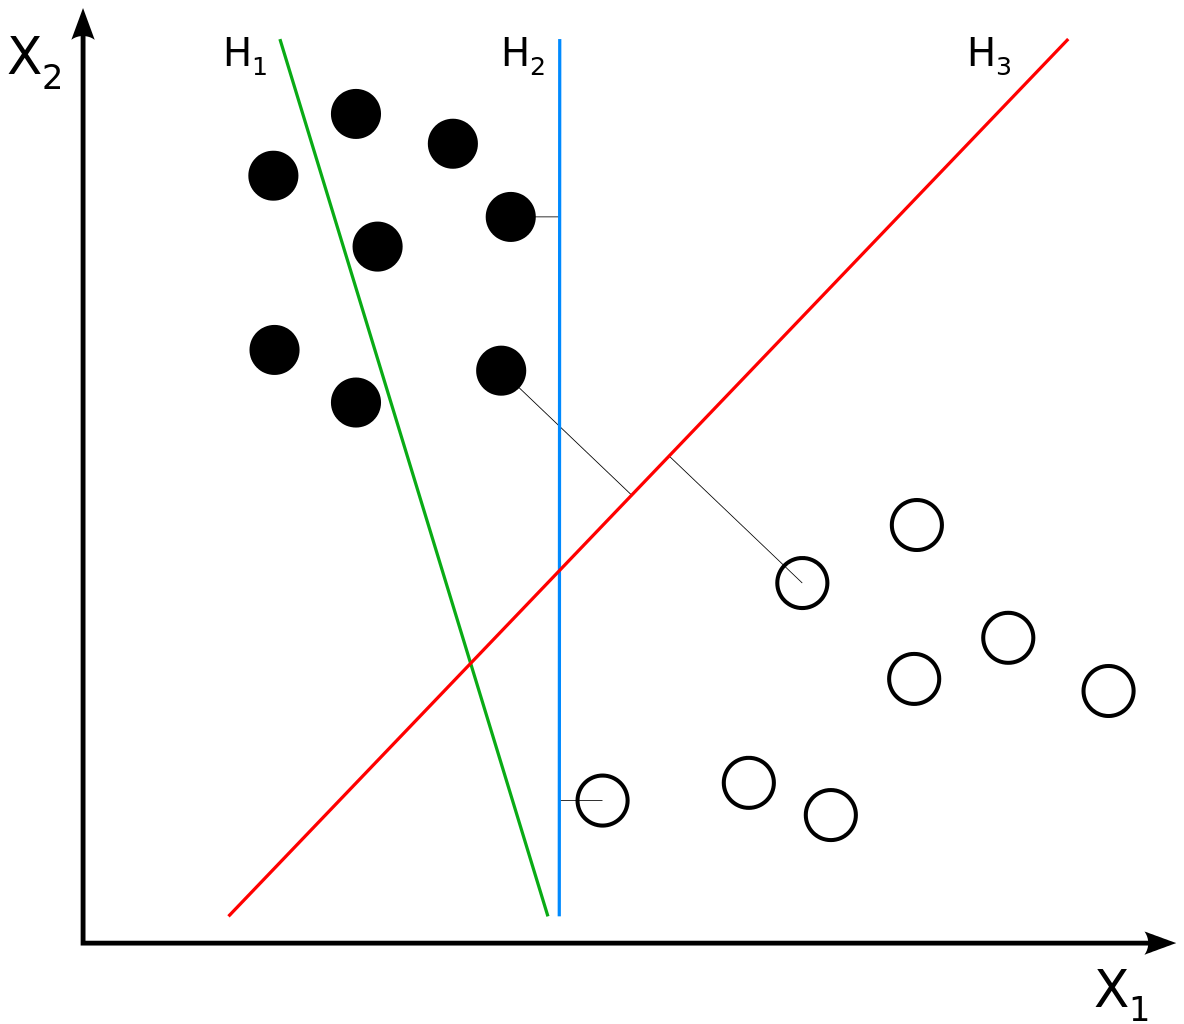
\includegraphics[scale = 0.15]{pics/SVM.png}
        \end{figure}

\item $H_3$ separa las clases con el margen máximo.

\end{itemize}


\subsection{Lingüística y Procesamiento del Lenguaje Natural (PNL)}

El conocimiento de las estructuras lingüísticas es fundamental para el diseño de características y el análisis de errores en el Procesamiento del Lenguaje Natural (PNL). Los enfoques de aprendizaje automático en PNL se basan en características que describen y generalizan las instancias de uso del lenguaje. El conocimiento lingüístico orienta la selección y el diseño de estas características, ayudando al algoritmo de aprendizaje automático a encontrar correlaciones entre el uso del lenguaje y las etiquetas objetivo \cite{bender2013linguistic}.

\begin{itemize}
  \item El conocimiento de las estructuras lingüísticas es importante para el diseño de características y el análisis de errores en PNL \cite{bender2013linguistic}.
  \item Los enfoques de aprendizaje automático en PNL requieren características que puedan describir y generalizar el uso del lenguaje.
  \item El objetivo es guiar al algoritmo de aprendizaje automático para encontrar correlaciones entre el uso del lenguaje y el conjunto de etiquetas objetivo.
  \item El conocimiento sobre las estructuras lingüísticas puede influir en el diseño de características para los enfoques de aprendizaje automático en PNL.
\end{itemize}

El PNL plantea diversos desafíos, como los costos de anotación, las variaciones de dominio y la necesidad de actualizaciones continuas. La anotación manual requiere mucho trabajo y tiempo. Las variaciones de dominio implican aprender patrones diferentes para diferentes corpus de texto. Los modelos entrenados en un dominio pueden no funcionar bien en otro. Además, los modelos de PNL pueden volverse obsoletos a medida que el uso del lenguaje evoluciona con el tiempo.




\section{Etiquetar Datos en PLN}

\begin{itemize}
   \item \textbf{Costos de Anotación}: la anotación manual es \textbf{laboriosa} y \textbf{consume mucho tiempo}.
   \item \textbf{Variaciones de Dominio}: el patrón que queremos aprender puede variar de un corpus a otro (por ejemplo, deportes, política).

   \item ¡Un modelo entrenado con datos anotados de un dominio no necesariamente funcionará en otro!
   \item Los modelos entrenados pueden quedar desactualizados con el tiempo (por ejemplo, nuevos hashtags).
\end{itemize}

\paragraph{Variación de Dominio en el Análisis de Sentimiento}
\begin{enumerate}
   \item Para mí, la cola era bastante \textcolor[rgb]{0.00,0.00,1.00}{\textbf{pequeña}} y solo tuve que esperar unos 20 minutos, ¡pero valió la pena! :D @raynwise
   \item Extraña espacialidad en Stuttgart. La habitación del hotel es tan \textcolor[rgb]{1.00,0.00,0.00}{\textbf{pequeña}} que apenas puedo moverme, pero los alrededores son inhumanamente vastos y largos bajo construcción.
\end{enumerate}

\paragraph{Superando los costos de anotación de datos}
Supervisión Distant:
\begin{itemize}
   \item Etiquetar automáticamente datos no etiquetados (\textbf{API de Twitter}) utilizando un método heurístico.
   \item \textbf{Enfoque de Anotación de Emoticonos (EAA)}: los tweets con emoticonos positivos \textcolor[rgb]{0.00,0.00,1.00}{\textbf{:)}} o negativos \textcolor[rgb]{1.00,0.00,0.00}{\textbf{:(}} se etiquetan según la polaridad indicada por el emoticono~\cite{Read2005}.
   \item El emoticono se \textbf{elimina} del contenido.
   \item Este enfoque también se ha ampliado utilizando hashtags como \#anger y emojis.
   \item No es trivial encontrar técnicas de supervisión distante para todo tipo de problemas de PNL.
\end{itemize}

\paragraph{Crowdsourcing}
\begin{itemize}
   \item Confiar en servicios como \textbf{Amazon Mechanical Turk} o \textbf{Crowdflower} para solicitar a la \textbf{multitud} que anote datos.
   \item Esto puede resultar costoso.
   \item Es difícil garantizar la calidad de las anotaciones.
\end{itemize}

\section{Paradigmas de Aprendizaje Automático}

Hasta el año 2010, el Procesamiento del Lenguaje Natural (PLN) se basaba en modelos de aprendizaje poco profundos y en características manuales. Por ejemplo, en 2013, el taller de Evaluación Semántica (SemEval) organizó la tarea de ``Análisis de sentimientos en Twitter'' \cite{Semeval2013}. Esta tarea se dividió en dos sub-tareas: el nivel de expresión y el nivel del mensaje. El nivel de expresión se centró en determinar la polaridad del sentimiento de un mensaje según una entidad marcada dentro de su contenido, mientras que el nivel del mensaje buscaba determinar la polaridad según el mensaje en general. Los organizadores proporcionaron conjuntos de datos de entrenamiento y prueba para ambas tareas \cite{Semeval2013}.

El equipo que logró el mejor rendimiento en ambas tareas, entre 44 equipos participantes, fue el equipo llamado \emph{NRC-Canada} \cite{Mohammad2013}. Este equipo propuso un enfoque supervisado utilizando un clasificador SVM lineal, utilizando características hechas a mano para representar los tweets. Algunas de estas características fueron:

\begin{enumerate}
  \item N-gramas de palabras.
  \item N-gramas de caracteres.
  \item Etiquetas de partes del discurso.
  \item Agrupaciones de palabras entrenadas con el método de agrupamiento de Brown \cite{brown1992class}.
  \item El número de palabras alargadas (palabras con un carácter repetido más de dos veces).
  \item El número de palabras con todas las letras en mayúscula.
  \item La presencia de emoticonos positivos o negativos.
  \item El número de negaciones individuales.
  \item El número de secuencias contiguas de puntos, signos de interrogación y signos de exclamación.
  \item Características derivadas de lexicones de polaridad \cite{Mohammad2013}. Dos de estos lexicones se generaron utilizando el método PMI a partir de tweets anotados con hashtags y emoticonos.
\end{enumerate}

Hasta el año 2014, la mayoría de los sistemas de última generación en PLN se basaban en ingeniería de características junto con modelos de aprendizaje automático superficiales, como SVM y CRF. Diseñar las características de un sistema de PLN ganador requería un amplio conocimiento específico del dominio. El sistema desarrollado por el equipo NRC-Canada se construyó antes de que el aprendizaje profundo se volviera popular en el campo del PLN. Por otro lado, los sistemas de Aprendizaje Profundo, también conocidos como Deep Learning, se basan en redes neuronales para aprender automáticamente buenas representaciones.

El Aprendizaje Profundo ha proporcionado resultados de vanguardia en la mayoría de las tareas de PLN. Grandes cantidades de datos de entrenamiento y máquinas GPU multicore más rápidas son fundamentales para el éxito del aprendizaje profundo. Las redes neuronales y los vectores de palabras, también conocidos como word embeddings, desempeñan un papel fundamental en los modelos modernos de PLN.

\begin{figure}[h]
	\centering
	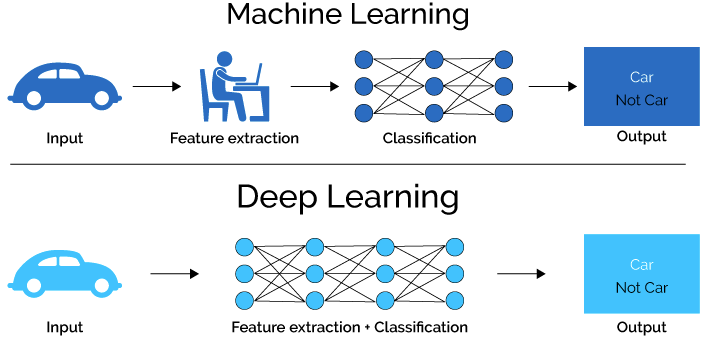
\includegraphics[scale=0.25]{pics/MLvsDL.png}
	\caption{Ingeniería de Características vs Aprendizaje Profundo}
	\label{fig:MLvsDL}
\end{figure}


\paragraph{Aprendizaje Profundo y Conceptos Lingüísticos}
Si los modelos de aprendizaje profundo pueden aprender representaciones automáticamente, ¿siguen siendo útiles los conceptos lingüísticos (por ejemplo, sintaxis, morfología)? Algunos defensores del aprendizaje profundo argumentan que estas propiedades lingüísticas inferidas y diseñadas manualmente no son necesarias, y que la red neuronal aprenderá estas representaciones intermedias (o equivalentes o mejores) por sí misma \cite{goldberg2016primer}. Aún no hay un consenso definitivo al respecto. Goldberg cree que muchos de estos conceptos lingüísticos pueden ser inferidos por la red por sí misma si se le proporciona suficiente cantidad de datos. Sin embargo, en muchos otros casos no disponemos de suficientes datos de entrenamiento para la tarea que nos interesa, y en estos casos proporcionar a la red los conceptos generales más explícitos puede ser muy valioso.

\section{Historia}

Los orígenes de PLN se remontan a los años 50 con el famoso test de Alan Turing: una máquina será considerada inteligente cuando sea capaz de conversar con una persona sin que esta pueda determinar si está hablando con una máquina o un ser humano. A lo largo de su historia la disciplina ha tenido tres grandes períodos: 1) el racionalismo, 2) el empirismo, y 3) el aprendizaje profundo [Deng y Liu, 2018] que describimos a continuación.

El racionalismo abarca desde 1950 a 1990, donde las soluciones consistían en diseñar reglas manuales para incorporar mecanismos de conocimiento y razonamiento. Un ejemplo emblemático es el agente de conversación (o chatbot) ELIZA desarrollado por Joseph Weizenbaum que simulaba  un psicoterapeuta rogeriano. Luego, a partir de la década de los 90s, el diseño de métodos estadísticos y de aprendizaje automático construidos sobre corpus llevan a PLN hacia un enfoque empirista. Las reglas ya no se construyen sino que se “aprenden” a partir de datos etiquetados.  Algunos modelos representativos de esta época son los filtros de spam basados en modelos lineales, las cadenas de Markov ocultas para la extracción de categorías sintácticas y los modelos probabilísticos de IBM para la traducción automática. Estos modelos se caracterizaban por ser poco profundos en su estructura de parámetros y por depender de características manualmente diseñadas para representar la entrada.

A partir del año 2010, las redes neuronales artificiales, que son una familia de modelos de aprendizaje automático, comienzan a mostrar resultados muy superiores en varias tareas emblemáticas de PLN [Collobert et al., 2011]. La idea de estos modelos es representar la entrada (el texto) con una jerarquía de parámetros (o capas) que permiten encontrar representaciones idóneas para la tarea en cuestión, proceso al cual se refiere como “aprendizaje profundo”. Estos modelos se caracterizan por tener muchos más parámetros que los modelos anteriores (superando la barrera del millón en algunos casos) y requerir grandes volúmenes de datos para su entrenamiento. Una gracia de estos modelos es que pueden ser pre-entrenados con texto no etiquetado como libros, Wikipedia, texto de redes sociales y de la Web para encontrar representaciones iniciales de palabras y oraciones (a lo que conocemos como word embeddings),  las cuales pueden ser posteriormente adaptadas para la tarea objetivo donde sí se tienen datos etiquetados (Proceso conocido como transfer learning). Aquí destacamos modelos como Word2Vec [Mikolov 2013], BERT  [Devlin 2018] y GPT-3  [Brown 2020].

Este tipo de modelos ha ido perfeccionándose en los últimos años, llegando a obtener resultados cada vez mejores para casi todos los problemas del área [NLPProgress]. Sin embargo, este progreso no ha sido libre de controversias. El  aumento exponencial en la cantidad de parámetros de cada nuevo modelo respecto a su predecesor, hace que los recursos computacionales y energéticos necesarios para construirlos sólo estén al alcance de unos pocos. Además, varios estudios han mostrado que estos modelos aprenden y reproducen los sesgos y prejuicios (ej: género, religión, racial) presentes en los textos a partir de los cuales se entrenan. Sin ir más lejos, la investigadora  Timmnit Gebru fue despedida de Google  cuando se le negó el permiso para publicar un artículo que ponía de manifiesto estos problemas [Bender 2021].


El progreso de la PNL se puede dividir en tres oleadas principales: 1) racionalismo, 2) empirismo y 3) aprendizaje profundo \cite{deng2018deep}.
\begin{itemize}
   \item [1950 - 1990] Racionalismo: se enfocaba en diseñar reglas hechas a mano para incorporar conocimiento y mecanismos de razonamiento en sistemas de PNL inteligentes (por ejemplo, ELIZA para simular a un psicoterapeuta Rogeriano, MARGIE para estructurar información del mundo real en ontologías de conceptos).
   \item [1991 - 2009] Empirismo: se caracteriza por la explotación de corpora de datos y modelos de aprendizaje automático y estadísticos (superficiales) (por ejemplo, Naive Bayes, HMMs, modelos de traducción IBM).
   \item [2010 - ] Aprendizaje Profundo: la ingeniería de características (considerada como un cuello de botella) se reemplaza con el aprendizaje de representaciones y/o redes neuronales profundas (por ejemplo, \url{https://www.deepl.com/translator}). Un artículo muy influyente en esta revolución: \cite{collobert2011natural}.
\end{itemize}

\footnotetext{Las fechas son aproximadas.}

\section{Conclusiones}


En este capítulo, hemos explorado el desafío de entender y producir lenguaje utilizando computadoras. El aprendizaje automático supervisado es una de las principales técnicas utilizadas para abordar este desafío. Además, hemos discutido las propiedades desafiantes del lenguaje, como la discreción, la composicionalidad y la dispersión. Estos aspectos nos muestran la complejidad inherente al procesamiento del lenguaje natural y nos desafían a encontrar soluciones efectivas.
